\documentclass[a4paper]{article}
\topmargin	-10mm
\oddsidemargin	0mm
\textwidth	150mm
\textheight	230mm

\newcommand{\ba}{ {\boldsymbol a} }
\newcommand{\bA}{ {\boldsymbol A} }
\newcommand{\bb}{ {\boldsymbol b} }
\newcommand{\bB}{ {\boldsymbol B} }
\newcommand{\bc}{ {\boldsymbol c} }
\newcommand{\bC}{ {\boldsymbol C} }
\newcommand{\bd}{ {\boldsymbol d} }
\newcommand{\bD}{ {\boldsymbol D} }
\newcommand{\be}{ {\boldsymbol e} }
\newcommand{\bE}{ {\boldsymbol E} }
\newcommand{\boldf}{ {\boldsymbol f} }
\newcommand{\bF}{ {\boldsymbol F} }
\newcommand{\bg}{ {\boldsymbol g} }
\newcommand{\bG}{ {\boldsymbol G} }
\newcommand{\bh}{ {\boldsymbol h} }
\newcommand{\bH}{ {\boldsymbol H} }
\newcommand{\bi}{ {\boldsymbol i} }
\newcommand{\bI}{ {\boldsymbol I} }
\newcommand{\bj}{ {\boldsymbol j} }
\newcommand{\bJ}{ {\boldsymbol J} }
\newcommand{\bk}{ {\boldsymbol k} }
\newcommand{\bK}{ {\boldsymbol K} }
\newcommand{\bl}{ {\boldsymbol l} }
\newcommand{\bL}{ {\boldsymbol L} }
\newcommand{\bm}{ {\boldsymbol m} }
\newcommand{\bM}{ {\boldsymbol M} }
\newcommand{\bn}{ {\boldsymbol n} }
\newcommand{\bN}{ {\boldsymbol N} }
\newcommand{\bo}{ {\boldsymbol o} }
\newcommand{\bO}{ {\boldsymbol O} }
\newcommand{\bp}{ {\boldsymbol p} }
\newcommand{\bP}{ {\boldsymbol P} }
\newcommand{\bq}{ {\boldsymbol q} }
\newcommand{\bQ}{ {\boldsymbol Q} }
\newcommand{\br}{ {\boldsymbol r} }
\newcommand{\bR}{ {\boldsymbol R} }
\newcommand{\bs}{ {\boldsymbol s} }
\newcommand{\bS}{ {\boldsymbol S} }
\newcommand{\bt}{ {\boldsymbol t} }
\newcommand{\bT}{ {\boldsymbol T} }
\newcommand{\bu}{ {\boldsymbol u} }
\newcommand{\bU}{ {\boldsymbol U} }
\newcommand{\bv}{ {\boldsymbol v} }
\newcommand{\bV}{ {\boldsymbol V} }
\newcommand{\bw}{ {\boldsymbol w} }
\newcommand{\bW}{ {\boldsymbol W} }
\newcommand{\bx}{ {\boldsymbol x} }
\newcommand{\bX}{ {\boldsymbol X} }
\newcommand{\by}{ {\boldsymbol y} }
\newcommand{\bY}{ {\boldsymbol Y} }
\newcommand{\bz}{ {\boldsymbol z} }
\newcommand{\bZ}{ {\boldsymbol Z} }
\newcommand{\vc}[1]{\mbox{\boldmath $1$}}
\newcommand{\balph}{ {\boldsymbol \alpha} }
\newcommand{\balpha}{ {\boldsymbol \alpha} }
\newcommand{\bbet}{ {\boldsymbol \beta} }
\newcommand{\bbeta}{ {\boldsymbol \beta} }
\newcommand{\bgam}{ {\boldsymbol \gamma} }
\newcommand{\bgamma}{ {\boldsymbol \gamma} }
\newcommand{\bGamma}{ {\boldsymbol \Gamma} }
\newcommand{\bdelta}{ {\boldsymbol \delta} }
\newcommand{\bDelta}{ {\boldsymbol \Delta} }
\newcommand{\beps}{ {\boldsymbol \epsilon} }
\newcommand{\bepsilon}{ {\boldsymbol \epsilon} }
\newcommand{\bphi}{ {\boldsymbol \phi} }
\newcommand{\bPhi}{ {\boldsymbol \Phi} }
\newcommand{\bpi}{ {\boldsymbol \pi} }
\newcommand{\bpsi}{ {\boldsymbol \psi} }
\newcommand{\bkap}{ {\boldsymbol \kappa} }
\newcommand{\bkappa}{ {\boldsymbol \kappa} }
\newcommand{\bKappa}{ {\boldsymbol \Kappa} }
\newcommand{\blam}{ {\boldsymbol \lambda} }
\newcommand{\blambda}{ {\boldsymbol \lambda} }
\newcommand{\bLambda}{ {\boldsymbol \Lambda} }
\newcommand{\bmu}{ {\boldsymbol \mu} }
\newcommand{\bMu}{ {\boldsymbol \Mu} }
\newcommand{\bet}{ {\boldsymbol \eta} }
\newcommand{\bome}{ {\boldsymbol \omega} }
\newcommand{\bomega}{ {\boldsymbol \omega} }
\newcommand{\bOmega}{ {\boldsymbol \Omega} }
\newcommand{\bnabla}{ {\boldsymbol \nabla} }
\newcommand{\brho}{ {\boldsymbol \rho} }
\newcommand{\bsigma}{ {\boldsymbol \sigma} }
\newcommand{\bSig}{ {\boldsymbol \Sigma} }
\newcommand{\bSigma}{ {\boldsymbol \Sigma} }
\newcommand{\btheta}{ {\boldsymbol \theta} }
\newcommand{\bTheta}{ {\boldsymbol \Theta} }
\newcommand{\bzeta}{ {\boldsymbol \zeta} }
\newcommand{\bPsi}{ {\boldsymbol \Psi} }
\newcommand{\btau}{ {\boldsymbol \tau} }
\newcommand{\bzero}{ {\boldsymbol 0} }
\newcommand{\bones}{ {\boldsymbol 1} }
\newcommand{\given}{\,|\,}
\newcommand{\sS}{{\cal S}}
\newcommand{\Ss}{{\cal S}}
\newcommand{\Field}{{\cal F}}
\newcommand{\colsp}{{\cal C}}
\newcommand{\nullsp}{{\cal N}}
\newcommand{\rowsp}{{\cal R}}
\newcommand{\tildeC}{\tilde{C}}
\newcommand{\tildeK}{\tilde{K}}
\newcommand{\tildew}{\tilde{w}}
\newcommand{\tildebw}{\tilde{\bw}}
\newcommand{\tildebW}{\tilde{\bW}}
\newcommand{\calC}{{\cal C}}
\newcommand{\calcbC}{{\bf {\cal C}}}

\def\rx{{\texttt{T-REX\ }}}
\def\rxe{{\texttt{T-REX}}}
\def\du{{\texttt{DUNE}\ }}
\def\due{{\texttt{DUNE}}}

% == Maths
\usepackage{amssymb}
\usepackage{amsmath}
\usepackage{graphicx}
\usepackage{enumitem}
\usepackage{xcolor}
\usepackage[normalem]{ulem} %to strike the words

\usepackage{float}
\usepackage{cleveref}

\newcounter{reviewer}
\def\revcom{\textbf{Reviewer comment}}
\def\aecom{\textbf{Associate Editor comment }}
\def\reply{\textbf{Reply}}
\def\action{\textbf{Action}}

\newlist{answers}{enumerate}{10}
\setlist[answers]{leftmargin=*, label=\arabic{reviewer}.\arabic*}

\newcommand{\edcomment}[1]{{\color{green}{\{Editor: 1\}}}}
\newcommand{\frevcomment}[1]{{\color{blue}{\{Rev 1: 1\}}}}
\newcommand{\srevcomment}[1]{{\color{red}{\{Rev 2: 1\}}}}
\newcommand{\trevcomment}[1]{{\color{violet}{\{Rev 3: 1\}}}}

\usepackage{amsthm,amsmath,natbib}
\RequirePackage[colorlinks,citecolor=blue,urlcolor=blue]{hyperref}

\begin{document}

%----------------------------------------------------------------------
\title{Autonomous Oceanographic Data Collection. Learning Excursion Sets of Vector-valued Gaussian Random Fields
  \\\vspace{5mm}
 Authors response to 2$^{nd}$ review
  \\\vspace{5mm}
\small{Manuscript: AOAS1910-027}}
\author{ }

\date{\today}

\maketitle

We are grateful to the editors and reviewers for their comments and suggestions. They have all been considered in this revised version of our manuscript. The changes in the manuscript are reflected in the points shown below.\\

\par \vspace{1em}


%======================================================================
\section*{Editor}
%======================================================================
All comments of the Editor are listed below and answered on a point-by-point basis.

\vspace{5mm}
\noindent {\bf{1. Sampling limitations:}} You explained in your response file (R1S3.pdf) the limitations of the sampling design (comment 4 from the AE's previous review). I agree with the AE (bullet 1, R2AE2.pdf) that some (perhaps slightly abbreviated) version of your response on p4 (middle) would be important to include; viz.

\begin{quote}
"The sampling capabilities are restricted by the sensors onboard the AUV, the computational load, and navigation resources. The sampling of temperature and salinity variables can be much higher than the grid resolution, but, due to computational and navigation resources available on the AUV, assimilation into a discretized fixed grid is necessary.`` 
\end{quote}


\reply: We agree, and we have addressed this point as you suggest. For more details, see \aecom \textbf{1}. 
 
\vspace{5mm}
\noindent {\bf{2. Variance of errors:}} In view of the apparent nugget effects of 0.42 and 0.7 for salinity
and temperature, respectively, in Fig 9(c) (p21), I confess to being
a little puzzled myself by this statement on p22:
"We specify variance $0.25^2$ for both errors, which is based on a
middle ground between the nugget effect in the empirical variogram
and the sensor specifications."  Is 0.0625 really a "middle ground"?
Or, did you have other reasons for choosing 0.0625 not stated here?
In any event, I agree with the AE (bullet 5): "either give a better
justification of your choice of 0.0625 or, if that’s not possible,
then redo the analysis with a more justifiable choice."

\vspace{5mm}
\reply: We have revised the text specification of model parameters. In the revised version we have a plot with analysis of survey sampling residuals at the end of the paper. This shows that the specified nugget effect and other parameters are reasonable, but it is of course a simplification of the complex ocean. We believe this part fits as an honest discussion at the end of the results section. We have addressed this point further in \aecom \textbf{5}. 

\vspace{5mm}
\noindent {\bf{3. Exposition:}} Apart from corrections noted by the AE (bullets 2,3,4,6), Referee 1
offered suggestions on shortening. Neither the AE nor I feel that re-structuring is needed.  In fact, some of the Referee's proposed changes would not be even desirable, from my perspective: I would not want you to "Consider putting the background material in an appendix to go as supplementary material" because, in my opinion, this background material is essential. And the simulation section (design and results) is already quite efficient. I include the Referee's report (R2R5.pdf) primarily for your information (the remarks from Ehrenberg are worth reading).

\vspace{5mm}
\reply: We agree that the remarks of Ehrenberg are very useful! Regarding the structure, we seriously considered your suggestions about the background in supplementary material, but in the end thought it was too much of a reduction to go through with. It would be very difficult to grasp the applied contribution of our paper if the background parts were in the supplemental material, and only some readers take the extra effort of reading that. Based on the report of the reviewer, we did however go through the background and cut a few unnecessary formulations in the revised version.

\vspace{5mm}
\noindent {\bf{4. Figures:}} Like most journals, AOAS discourages the use of color in figures,
unless absolutely essential for reader comprehension.  I believe
that color is important for Figures 1, 2, 4, 11 and perhaps 5 and 6.
But color is not even mentioned in the caption for Figure 3; your
different line types likely will suffice in Figures 8 and 9; and
probably nothing will be lost if Figures 7 and 10 were black-and-white.
Color is very expensive to print, so we appreciate your attention
to this cost-saving measure.

\vspace{5mm}
\reply: We agree on all your points here, except Fig.8. Line type will be tricky for Fig. 8, when lines are very close together especially in Fig.8b, and Fig.8c. So we ask to consider that this figure is kept in color. Revised Fig. 3 and 11 are in black-and-white. Fig. 4, 5, and 6 have been made with a black-and-white compatible color-map, so they can be converted to black-and-white.

\vspace{5mm}
\noindent {\bf{Other comments:}} In your revision, you may want to include in the
acknowledgements, p26, the conscientious efforts of the anonymous
reviewers, whose comments led to this favorable outcome.

\vspace{5mm}
\reply: We agree that this effort should be noted. We have added the following statement to the acknowledgements.

\begin{quote}
"We thank the anonymous reviewers for their careful reading of our manuscript and their many insightful comments and suggestions.``
\end{quote}

%======================================================================
 \section*{Associate Editor}
%======================================================================
All comments of the Associate Editor are listed below and answered on a point-by-point basis.

\setcounter{reviewer}{1}

\vspace{5mm}
\noindent \aecom \textbf{1 - Reply to AE comment 4}: 
I thank you for explaining the sampling limitations to me in your reply.  However, I think these limitations should also be noted in the narrative, and the sub-optimality of the resulting trajectory should be acknowledged.

\vspace{5mm}
\reply: We agree that this should be mentioned in the text. We have added the following text in the Closing remarks section at page 25.

\begin{quote}
    "The sampling capabilities are restricted by the sensors onboard the AUV, the computational load and navigation resources. The sampling of temperature and salinity variables can be much higher than the grid resolution, but, due to computational and navigation resources available on the AUV, assimilation into a discretized fixed grid is necessary.``
\end{quote}

\vspace{5mm}
\noindent \aecom \textbf{2 - Page 2, line 15}:  I think it would be more appropriate to refer to this as sampling design rather than sampling.

\vspace{5mm}
\reply: We have removed the word sampling from the sentence. It now reads:

\begin{quote}
    "Models and methods from spatial statistics and experimental design can clearly contribute to this challenge.``
\end{quote}

\vspace{5mm}
\noindent \aecom \textbf{3 - Page 4, line 3}:  Replace “proxys” with the correct plural “proxies”

\vspace{5mm}
\reply: Changed to “proxies” on page 4.

\vspace{5mm}
\noindent \aecom \textbf{4 - Page 5, line 16:}  Change  “the  PhD  thesis  (Stroh,  2018,  p.  82)”  to ”Stroh (2018, p. 82)”

\vspace{5mm}
\reply: We have changed the reference accordingly in the text at Page 5. 

\vspace{5mm}
\noindent \aecom \textbf{5 - Page 22, line 8:}  From Figure 9(c), the nugget effect in the empirical variogram appears to be approximately 0.4 for salinity and 0.7 for temperature.  Even if the sensor specifications were essentially 0, it would be a stretch to say that a variance of 0.0625 was a “middle ground” between the empirical nugget effect and the sensor specifications.  So either give a better justification of your choice of 0.0625 or, if that’s not possible, then redo the analysis with a more justifiable choice.

\vspace{5mm}
\reply: We have revised the text specification of model parameters in Sect. 4.1 and 4.2. The initial survey transect had no samples at very short distance, and these data are hence not reliable for extracting the nugget effect. The sensor-provided standard deviations of the measurement tools are in the fourth decimal points, but based on our experience \citep{fossuminformation}, there is more variability than this in temperature and salinity measurements in water samples close in space and time. This variability is partly due to dynamic water masses but also uncertainty in the AUV position. 
\begin{figure}[h] 
\centering
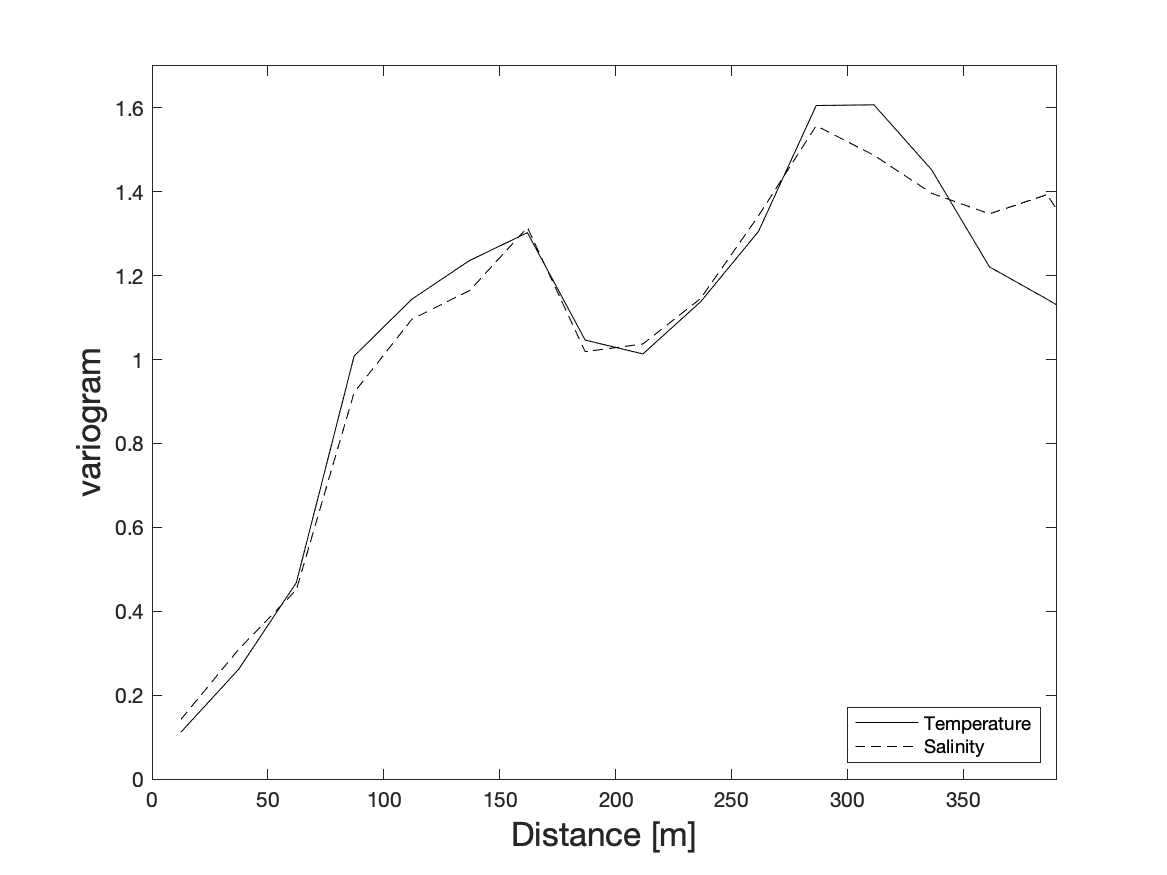
\includegraphics[width=0.6\textwidth]{Figures/field-trials/empVAR.png}
\caption{Empirical variogram of the scaled variables from the two runs. }
\label{empVar}
\end{figure}

In the revised manuscript, we made residual plots and empirical variograms for the actual survey data in Sect 4.3 (Figure 11 in the revised paper). In the two surveys, we have some samples close in space and it is possible to extract the nugget effect. These curves support our statements of a small but non-zero nugget (see Figure \ref{empVar}).

%One reason to keep a significant nugget effect here is to account for the dynamic water masses that are not captured in our model, but we expect this to be very small given our limited survey time, as was the case in \citep{fossuminformation}. Then again, between the two surveys, there is a change in the survey 1 and 2 paths caused by slightly different measurements at the two times of surveying. There could also be some uncertainty in the AUV location leading to samples not allocated to its true position. 

We further checked the sensitivity of the nugget specification in the sequential sampling algorithm. This was done by running synthetic cases of sampling paths and data up to a certain stage for different measurement noise variance levels. We see moderate changes in the sampling path patterns, but paths tend to be smoother for large nugget effect, as illustrated in Figure \ref{fig:nugget_comparison}.
Indeed, with small nugget (left display), the AUV reacts more to the observed temperature and salinity levels, and this leads to more small turns in its path.

We note that even though the sampling paths can be different, the posterior EPs in Figure \ref{fig:nugget_comparison} are similar and will thus lead to similar estimates for the ES. %We also remark that the differences in Figure \ref{fig:nugget_comparison} would get smaller if the sampling continues (here stopped for presentation purposes).

\begin{figure}[h]
    \centering
    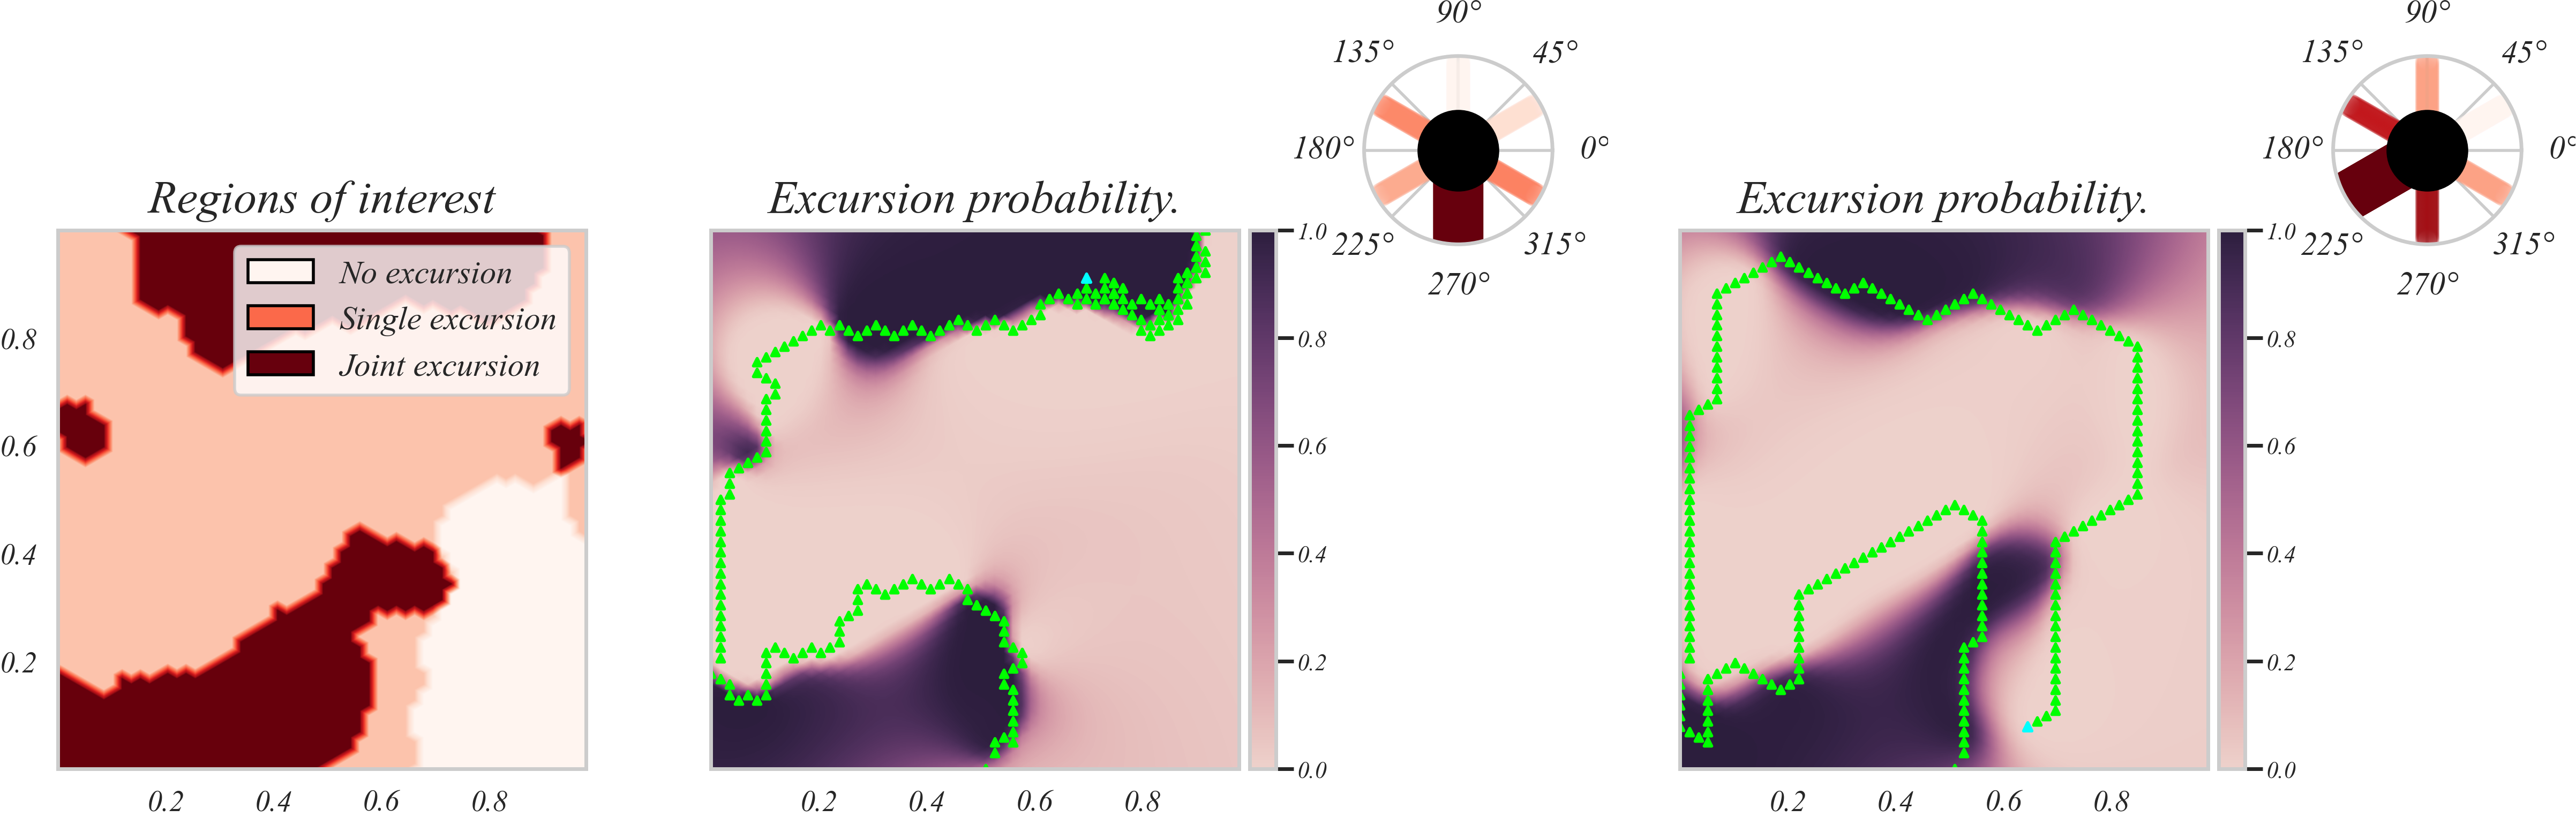
\includegraphics[scale=0.52]{ans_to_reviewers/merged_paths_2.png}
    \caption{Comparison of sampling paths and posterior EPs for different values of the measurement noise standard deviation (from left to right: $0.1$ and $0.5$). The sampling has been stopped after 200 steps.}
    \label{fig:nugget_comparison}
\end{figure}
In the revised manuscript we wrote two sentences around this sensitivity near Fig 10: 'The AUV paths in both runs are relatively
winding in the sense that the vehicle reacts to the data. In our
experience from simulations, the paths tend to be smoother when we
use larger measurement error variances for the AUV temperature and salinity observations. '

\vspace{5mm}
\noindent \aecom \textbf{6 - Page 22, line 5:}  Insert “triangular” immediately after “equilateral”

\vspace{5mm}
\reply: We have inserted this as suggested. 

\vspace{1em}


% == Adding references
\footnotesize
\bibliographystyle{apalike}
\bibliography{ref}

%=====================================================================
\end{document}
%=====================================================================
